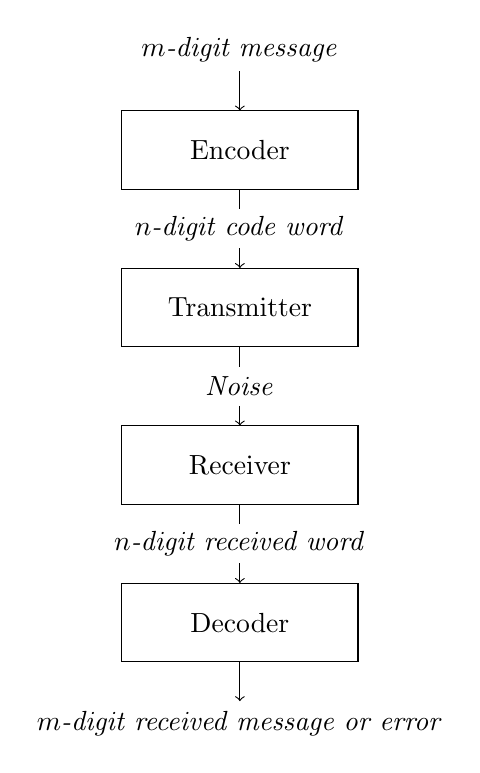
\begin{tikzpicture}[scale=1]

\draw [->] (0,8)  node [above] {\emph{$m$-digit message}} -- (0,7.5);

\node at (0,7) {Encoder};
\draw (-1.5,6.5) rectangle (1.5,7.5);
\draw (0,6.5)  -- (0,6.25);
\draw [->] (0,5.75)  -- (0,5.5);
\node at (0,6) {\emph{$n$-digit code word}};

\node at (0,5) {Transmitter};
\draw (-1.5,4.5) rectangle (1.5,5.5);
\draw (0,4.5)  -- (0,4.25);
\draw [->] (0,3.75)  -- (0,3.5);
\node at (0,4) {\emph{Noise}};

\node at (0,3) {Receiver};
\draw (-1.5,2.5) rectangle (1.5,3.5);
\draw (0,2.5)  -- (0,2.25);
\draw [->] (0,1.75)  -- (0,1.5);
\node at (0,2) {\emph{$n$-digit received word}};

\node at (0,1) {Decoder};
\draw (-1.5,0.5) rectangle (1.5,1.5);
\draw [->] (0,0.5)  -- (0,0) node [below] {\emph{$m$-digit received message or error}};

\end{tikzpicture}
